%% Interface-normal velocity extension for Eulerian level-set advection.
%% SKELETON -- parallel structure to the semi-Lagrangian article; figures/tables are
%% the single data source in ./data (regenerated by the Snakemake studies). The prose
%% of the results/discussion is to be written; the scaffold + data wiring compile now.
%% Build:  latexmk -pdf velocityExtension.tex
\documentclass[preprint,3p,11pt]{elsarticle}

\usepackage[T1]{fontenc}
\usepackage{amsmath,amssymb}
\usepackage{bm}
\usepackage{graphicx}
\usepackage{booktabs}
\usepackage{subcaption}
\usepackage{url}
\usepackage[hidelinks]{hyperref}

\graphicspath{{data/figures/}}
\journal{a computational physics journal}

\begin{document}

\begin{frontmatter}
\title{Interface-normal velocity extension for Eulerian level-set advection on
       unstructured meshes}
\author[tud]{Tomislav Mari\'c}
\ead{maric@mma.tu-darmstadt.de}
\address[tud]{Mathematical Modeling and Analysis, Technische Universit\"at Darmstadt, Germany}

\begin{abstract}
% TODO (skeleton): when a level set is advected by a velocity that is only physically
% meaningful at the interface, the field off the interface must be defined by an
% extension. This article studies interface-normal velocity-extension models for
% Eulerian level-set transport on unstructured finite-volume meshes, their effect on
% the transported interface accuracy and the level-set regularity, and their runtime-
% selectable implementation in OpenFOAM. Companion line to the semi-Lagrangian
% advection method (separate article).
Placeholder abstract -- see the semi-Lagrangian article for the companion method.
\end{abstract}

\begin{keyword}
level set \sep velocity extension \sep interface advection \sep unstructured meshes \sep OpenFOAM
\end{keyword}
\end{frontmatter}

% =============================================================================
\section{Introduction}
\label{sec:intro}
% TODO: motivate velocity extension for level-set transport with an interface-only
% velocity; contrast with the semi-Lagrangian characteristic advection (companion
% article); state the contribution (a runtime-selectable family of extension models
% + their verification on unstructured meshes).

\section{Velocity-extension models}
\label{sec:models}
% TODO: the runtime-selectable extension family --
%   none, anisotropicDiffusion, pseudoTime, steadyUpwind, closestPoint, meshWave.
% Give each model's formulation + the anchor-layer boundary treatment.

\section{Verification}
\label{sec:verification}
% TODO: reversed vortex / shear cases; convergence of the shape error and the
% narrow-band |grad psi| regularity per extension model; the static (t=0) extension
% test. Figures/tables below are the single data source in ./data (regenerated by the
% Snakemake studies with theme = velocity-extension).
\begin{figure}[t]
  \centering
  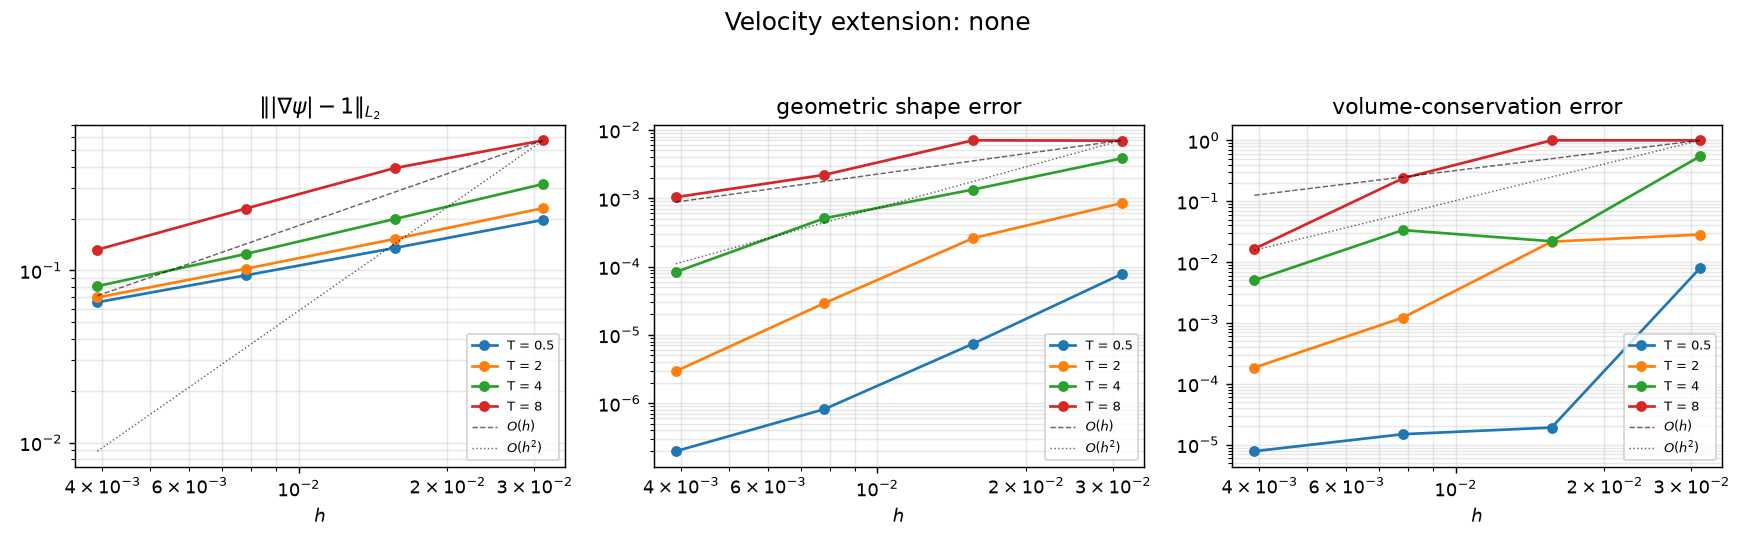
\includegraphics[width=0.7\linewidth]{convergence_none.png}
  \caption{Placeholder: convergence of the shape error for the baseline (no extension)
  case. Replace/extend with the per-model comparison once the studies are re-run
  through the thematic pipeline.}
  \label{fig:conv}
\end{figure}
% Data-driven table (generated when the VE studies run through the pipeline):
% \input{data/tables/ve_convergence_orders.tex}

\section{Conclusions}
\label{sec:conclusions}
% TODO.

\section*{Reproducibility}
Figures and tables are generated by the Snakemake velocity-extension studies and
written to \texttt{docs/velocity-extension/velocity-extension-article/data/};
\texttt{make studies \&\& make docs} reproduces them.

% \bibliographystyle{elsarticle-num}
% \bibliography{refs}

\end{document}
